% Metódy inžinierskej práce

\documentclass[10pt,twoside,slovak,a4paper]{article}

\usepackage[slovak]{babel}
%\usepackage[T1]{fontenc}
\usepackage[IL2]{fontenc} % lepšia sadzba písmena Ľ než v T1
\usepackage[utf8]{inputenc}
\usepackage{graphicx}
\usepackage{url} % príkaz \url na formátovanie URL
\usepackage{hyperref} % odkazy v texte budú aktívne (pri niektorých triedach dokumentov spôsobuje posun textu)

\usepackage{cite}
%\usepackage{times}

\pagestyle{headings}

\title{Virtuálna realita.\thanks{Semestrálny projekt v predmete Metódy inžinierskej práce, ak. rok 2022/23, vedenie: Bey Veronika}} % meno a priezvisko vyučujúceho na cvičeniach

\author{Bey Veronika\\[2pt]
	{\small Slovenská technická univerzita v Bratislave}\\
	{\small Fakulta informatiky a informačných technológií}\\
	{\small \texttt{xbey@stuba.sk}}
	}

\date{\small 05. october 2022} % upravte



\begin{document}

\maketitle

\begin{abstract}
\ldots
\end{abstract}



\section{Prečo tato tema?}


Túto tému som si vybrala, pretože je momentálne aktuálna. V súčasnosti existuje veľa hier, ktoré využívajú technológie virtuálnej reality. Je to jednoduchý a skvelý spôsob, ako zažiť emócie skutočného sveta bez toho, aby ste opustili svoj domov~\ref{nejaka}.



\section{Čo je virtuálna realita. A ako je to užitočné?} \label{nejaka}
.~\ref{f:rozhod} Prilby a technológie virtuálnej reality
\begin{figure*}[tbh]
\centering
%\includegraphics[scale=1.0]{diagram.pdf}
Virtuálna realita je akási podoba sveta okolo nás, umelo vytvorené pomocou technických prostriedkov a prezentované v digitálnej podobe. Vytvorené efekty sa premietajú do ľudskej mysle a umožňujú mu zažiť vnemy, ktoré sa čo najviac približujú skutočnosti \texttt{\%}).
\label{f:rozhod}
\end{figure*}



\section{Iná časť} \label{ina}

 Problém je v správnej implementácii virtuálneho prostredia. Oneskorenie a rozmazanie obrazu často vedú k závratom a nevoľnosti pri ponorení do virtuálnej reality.  Jednou z príčin nevoľnosti pri ponorení do virtuálnej reality je „klamanie“ mozgu. Poloha a pohyb človeka v priestore je fixovaný vestibulárnym aparátom umiestneným vo vnútornom uchu. Práve tento orgán prenáša do mozgu informácie o tom, čo sa s telom momentálne deje. Spolu s informáciami prijatými inými zmyslami (najmä očami) mozog určuje, čo zvyšok tela potrebuje robiť a cítiť.\cite{Coplien:MPD},Vo virtuálnej realite sa ukazovatele vestibulárneho aparátu a orgánov videnia líšia, pretože človek vidí pohyb, ale telo zostáva v pokoji. Mozog vníma vizuálnu informáciu ako halucináciu, ktorú možno zažiť pri otrave, a preto spôsobuje nevoľnosť, aby sa telo očistilo. Tento jav sa nazýva kinetóza.~\cite{Czarnecki:Staged, Czarnecki:Progress}. Napriek tomu, aj dnes na webe narazíme na všelijaké pochybné názory\cite{PLP-Framework}. Dôležité veci možno \emph{zdôrazniť kurzívou}.
\begin{figure}[h]
	\centering
	\scalebox{0.9}{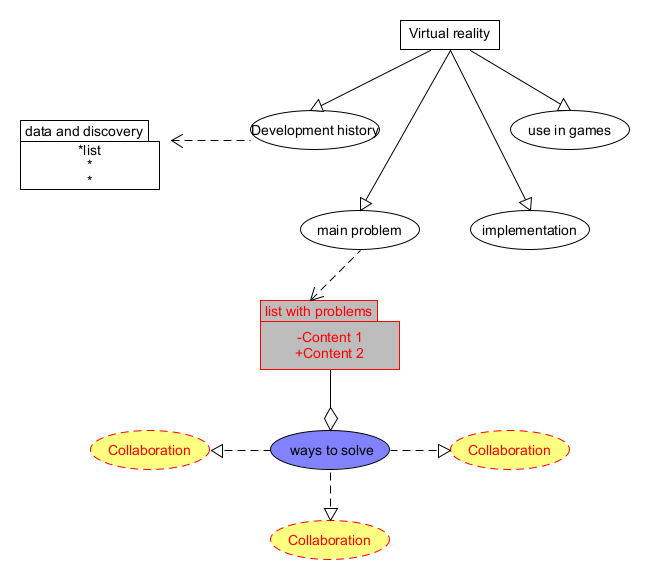
\includegraphics{pic1.jpg}} 
	\caption{Diagram}
	\label{framework}
\end{figure}


\subsection{Nejaké vysvetlenie} \label{ina:nejake}

Niekedy treba uviesť zoznam:

\begin{itemize}
\item jedna vec
\item druhá vec
	\begin{itemize}
	\item x
	\item y
	\end{itemize}
\end{itemize}

Ten istý zoznam, len číslovaný:

\begin{enumerate}
\item jedna vec
\item druhá vec
	\begin{enumerate}
	\item x
	\item y
	\end{enumerate}
\end{enumerate}


\subsection{Ešte nejaké vysvetlenie} \label{ina:este}

\paragraph{Veľmi dôležitá poznámka.}
Niekedy je potrebné nadpisom označiť odsek. Text pokračuje hneď za nadpisom.



\section{Dôležitá časť} \label{dolezita}




\section{Ešte dôležitejšia časť} \label{dolezitejsia}




\section{Záver} \label{zaver} % prípadne iný variant názvu



%\acknowledgement{Ak niekomu chcete poďakovať\ldots}


% týmto sa generuje zoznam literatúry z obsahu súboru literatura.bib podľa toho, na čo sa v článku odkazujete
\bibliography{literatura}
\bibliographystyle{plain} % prípadne alpha, abbrv alebo hociktorý iný
\end{document}
